% Thesis title page
\newcommand{\jadafont}[1]{{\fontfamily{pzc}\selectfont {\large #1}}}

\begin{titlepage}
\begin{center}
    {\large AUTOMATED ANSWER PAPER EVALUATION USING DEEP LEARNING AND NATURAL LANGUAGE PROCESSING\par}
    \vspace{50px}
	{\LARGE A Project Preliminary Report }\\\medskip
	%{ on }\\\bigskip
	%  \\	
\vspace{20px}
    Submitted by\\
    \vspace{20px}
    \begin{table}[!h]
\centering
\begin{tabular}{lc}
\underline{Name} & \underline{University Register No.} \\
\\
Pranav T. N. & KNR16CS046 \\
Rahul Mohanan A. K. & KNR16CS047 \\
Sourabh Subhod & KNR16CS053 \\
Vishal V. & KNR16CS059 \\
\end{tabular}
\end{table}
\vspace{15px}
to\\
\vspace{15px}
{\sc the A. P. J. Abdul Kalam Technological University\\
\vspace{10px}
in partial fulfillment of the requirements \\
\vspace{10px}
for the award of the Degree of}\\
\vspace{10px}
{\jadafont{Bachelor of Technology}\\\medskip
	{\sc in \\ Computer Science and Engineering} 

\vspace{.75cm}
      \vspace*{10pt}
        \centerline{
\includegraphics [keepaspectratio=true, scale=.3]{gcek.eps}}


\vspace{.6cm}
		  {{\sc Department of Computer Science and Engineering}}\\
		  {\bf \MakeUppercase{Government College  of Engineering Kannur}}\\ 
		  {\bf Kannur District, Kerala State}\\
	          {\bf November 2019}
}
\end{center}
\end{titlepage}
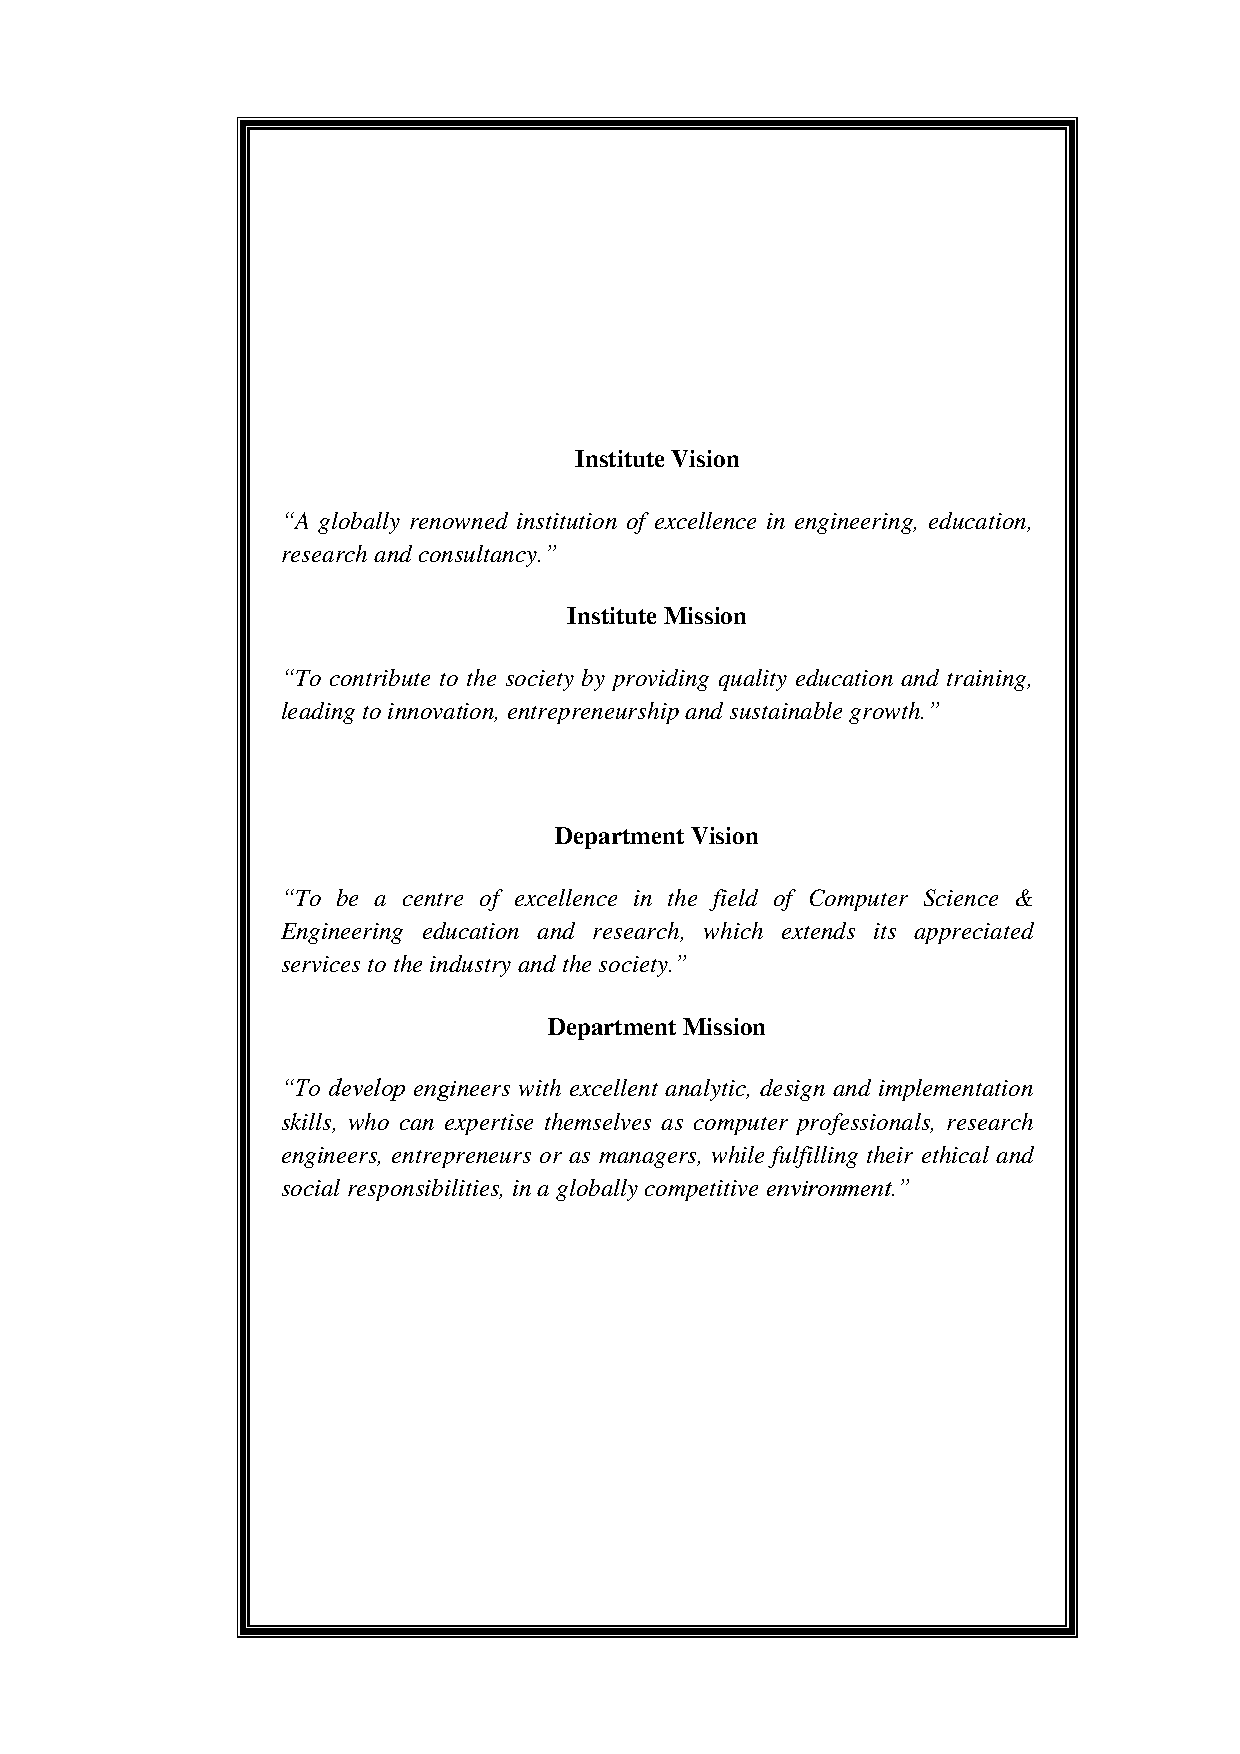
\includepdf[pages=1]{vision.pdf}
\cleardoublepage


% CERTIFICATE PAGE
%================
\begin{center}
     { {\sc Department. of Computer Science and Engineering}}\\
     {\bf \MakeUppercase{Government College  of Engineering Kannur}}\\
     {\bf Kannur District, Kerala State}\\ \bigskip   
        
      \vspace*{25pt}
      \centerline{
\includegraphics [keepaspectratio=true, scale=.2]{gcek.jpg}}
      \vspace*{2cm}
      \textbf{\large \jadafont{CERTIFICATE}}
      \vspace*{1cm}     
\end{center}

\begin{flushright}
{\today}\\ \bigskip                                  
\end{flushright}

\jadafont
  {~~Certified that this  is a bonafide record of the 
  {\em Project Preliminary work} done by the students whose 
  names are given below, with the title 
  ``{{\sc \normalsize AUTOMATED ANSWER PAPER EVALUATION USING 
  DEEP LEARNING AND NATURAL LANGUAGE PROCESSING}}'' towards 
  the partial fulfillment of the 
  requirements for the award of the Degree of Bachelor of Technology in Computer Science and Engineering of the 
  Department of Computer Science and Engineering under A. P. J. Abdul Kalam Technological University
  during the year 2019-2020.
  }

\begin{table}[!h]
\centering
\begin{tabular}{lc}
\underline{Name} & \underline{University Register No.} \\
\\
Pranav T. N. & KNR16CS046 \\
Rahul Mohanan A. K. & KNR16CS047 \\
Sourabh Subhod & KNR16CS053 \\
Vishal V. & KNR16CS059 \\
\end{tabular}
\end{table}

  
\vspace*{2.6cm}
\hspace*{-.5in}
\parbox{2.1in}{
\noindent {\bf Prof. Sajith B.} \\
\noindent {Project Guide}
}
 \parbox{2.1in}{
 \noindent {\bf Prof. Baburaj K. V. } \\
 \noindent {Project Co-ordinator}
 }
\parbox{2.1in}{
\noindent  \\[0.18cm] 
\noindent {\bf Dr. Rafeeque P. C.} \\
\noindent {HoD, Dept. of CSE}\\
}
\vspace*{1cm}
\parskip 8pt
\clearpage  
  
